\documentclass[tikz,border=8pt]{standalone}
\usepackage{pgfplots}
\pgfplotsset{compat=1.18}
\usepackage{xcolor}

% Custom Palette
\definecolor{brandblue}{RGB}{30, 64, 175}   % MXFP4
\definecolor{brandpurple}{RGB}{109, 40, 217} % M2XFP4
\definecolor{brandgray}{RGB}{100, 116, 139} % MXFP8
\definecolor{brandgreen}{RGB}{5, 150, 105}  % MXFP4R (Winner)

\begin{document}
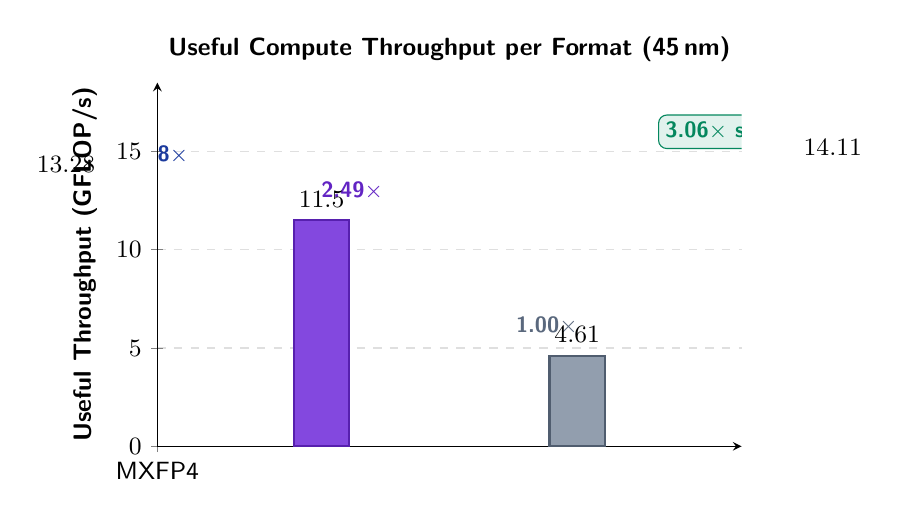
\begin{tikzpicture}
  \begin{axis}[
      ybar,
      bar width=20pt,
      width=9cm,
      height=6.2cm,
      enlarge x limits=0.18,
      symbolic x coords={MXFP4, M2XFP4, MXFP8, MXFP4R},
      xtick=data,
      xticklabels={MXFP4, M$^2$XFP4, MXFP8, \textbf{MXFP4R}},
      ylabel={Useful Throughput (GFLOP/s)},
      ymin=0, ymax=18.5,
      ymajorgrids=true,
      grid style={dashed, gray!25},
      axis lines=left,
      tick label style={font=\small\sffamily},
      label style={font=\small\sffamily\bfseries},
      title={\small\sffamily\textbf{Useful Compute Throughput per Format (45\,nm)}},
      title style={yshift=-2pt},
      nodes near coords,
      nodes near coords style={font=\small\sffamily\bfseries, yshift=1pt},
      every node near coord/.append style={
        /pgf/number format/fixed,
        /pgf/number format/precision=2
      }
    ]
    
    % Bars
    \addplot[draw=brandblue!80!black, fill=brandblue!85, thick] 
      coordinates {(MXFP4, 13.28)};
    \addplot[draw=brandpurple!80!black, fill=brandpurple!85, thick] 
      coordinates {(M2XFP4, 11.50)};
    \addplot[draw=brandgray!80!black, fill=brandgray!70, thick] 
      coordinates {(MXFP8, 4.61)};
    \addplot[draw=brandgreen!80!black, fill=brandgreen!90, thick] 
      coordinates {(MXFP4R, 14.11)};

    % Speedup badges above bars
    \node[font=\footnotesize\sffamily\bfseries, text=brandblue!90!black] at (axis cs:MXFP4, 14.8) {2.88$\times$};
    \node[font=\footnotesize\sffamily\bfseries, text=brandpurple!90!black] at (axis cs:M2XFP4, 13.0) {2.49$\times$};
    \node[font=\footnotesize\sffamily\bfseries, text=brandgray!90!black] at (axis cs:MXFP8, 6.1) {1.00$\times$};
    
    % Highlight badge for MXFP4R
    \node[draw=brandgreen!90!black, fill=brandgreen!12, rounded corners=3pt, inner sep=2.5pt, font=\footnotesize\sffamily\bfseries, text=brandgreen!90!black] 
      at (axis cs:MXFP4R, 16.0) {3.06$\times$ speedup};

  \end{axis}
\end{tikzpicture}
\end{document}
